%% content.tex
%%

%% ==============================
\chapter{Prelude}
\label{ch:Introduction}
%% ==============================

\section{Abstract}

\vspace*{\fill}
Die Strahlverfolgung und dazugehörige Techniken gewinnen gegenwärtig in der Echtzeitcomputergrafik an Bedeutung. Dabei haben bereits frühere Arbeiten
die blue noise Fehlerverteilungen miteinbezogen und deren Bedeutung in der Steigerung der wahrnehmbaren Bildqualität hervorgehoben und verdeutlicht.
Diese Arbeit wird diesen Stand aufnehmen und einen zeitlich stabilen Algorithmus erläutern. Ein Algorithmus, der mit Anzahl der Samples und Dimension
des Tracers einhergeht. Im Gegensatz zu vorhergehenden Ansätzen wollen wir direkt im Bildraum eine Fehlerumverteilung anwenden, um so eine entsprechend 
korrelierte Pixelfolge zu erhalten. All dies erreicht der Algorithmus ohne signifikanten Mehraufwand.
\vfill

\newpage

\section{Einleitung}

%% ==============
\chapter{Grundlagen}
\label{ch:Grundlagen}
%% ==============


%% ===========================
\section{Path Tracer}
\label{ch:Content1:sec:PathTracer}
\subsubsection{Funktionsweise}
In offline Produktionen bereits fest etabliert \cite{DisneyPathTracing} so gewinnt diese Technik
der Bilderzeugung durch neue Hardwareunterstützung für Echtzeitanwendungen an Aufmerksamkeit\cite{Sch19}.
Anstatt vom Objekt wird die Bilderzeugung ausgehend vom Betrachter angesetzt 
(siehe Abbildung\ref{pic::GrundkonzeptPathTracing}).
Bei der Bilderzeugung, ausgehend von Szenen, welche viel Geometrie beinhalten bzw. bei Szenen 
die generelle BRDF's verwenden eignet sich der \nameref{ch:Content1:sec:Path Tracer}.

\begin{figure}[H]
    \centering
    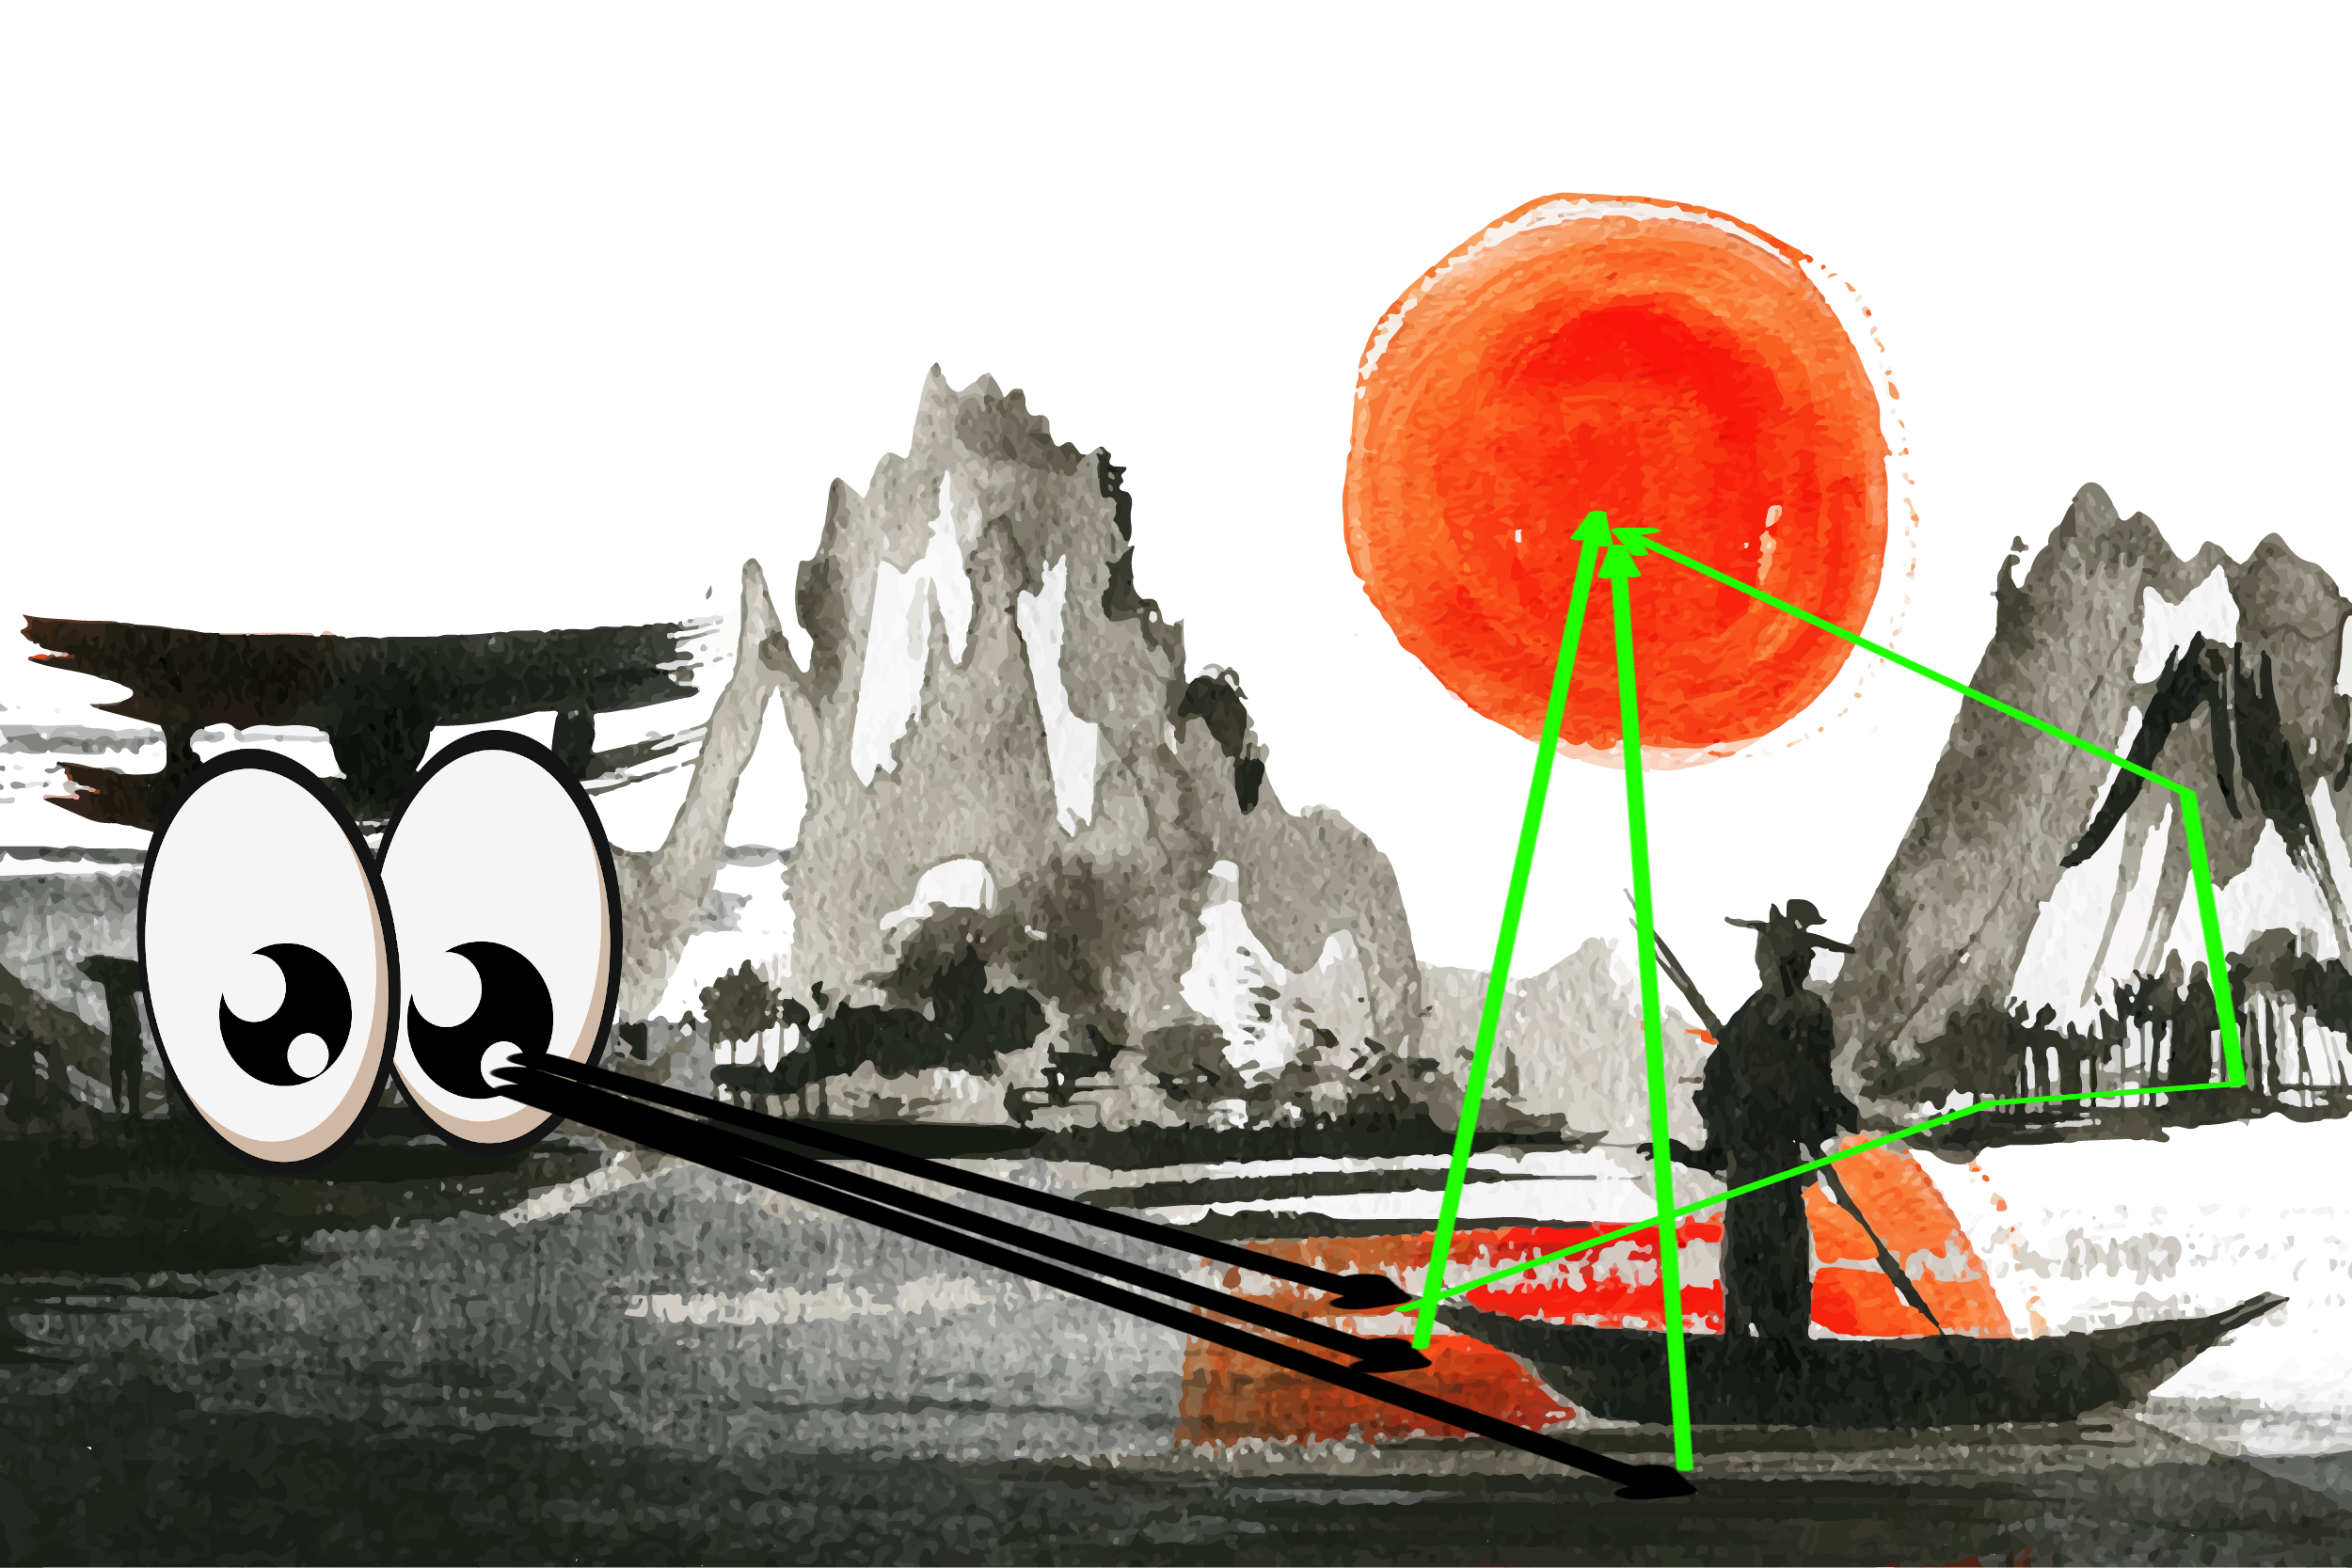
\includegraphics[width=\linewidth]{content/PathTracer/Bilder/PathTracerGuide.png}
    \caption{Grundkonzept Path Tracer}
    \label{pic::GrundkonzeptPathTracing}
\end{figure}

Der \nameref{ch:Content1:sec:Path Tracer} ist in Hinsicht der Beleuchtung komplett. Deshalb lässt sich damit
\textit{Global Illumination} erreichen. Der hier verwendete \nameref{ch:Content1:sec:Path Tracer} in 
\cite{Benty18} verwendet eine klassische Umsetzung.\par
Der Path Tracer beruht auf Erkenntnisse der Lösung der allgemeinen Rendergleichung.\nameref{eq:Allgemeine Rendergleichung}

\begin{equation}\label{eq:Allgemeine Rendergleichung}
    I(x,{x}^{'}) = g(x,{x}^{'}) * \biggl[\epsilon(x,{x}^{'}) + 
    \int_{S}^{} \rho(x,{x}^{'},{x}^{''})
    I({x}^{'},{x}^{''}d{x}^{''})\biggr] 
\end{equation}

Sie beschreibt den Energietransport \textit{I} von einem Punkt ${x}^{'}$
zu einem Punkt x. Dabei ist ein maßgebender Faktor der Geometrieterm \textit{g},
der die relative Lage der beiden Punkte zueinander im Raum beschreibt.
Ein weiterer Faktor ist die Abstrahlung \textit{$\epsilon$} von ${x}^{'}$ nach x. 
Beeinflusst wird der Energiefluss auch durch
die bidirektionale Verteilungsfunktion \textit{$\rho$}, welche Aufschluss über
das einfallende Licht von einem Punkt ${x}^{''}$ über ${x}^{'}$ zu x gibt.\par
Die Schlussfolgerung aus dieser Gleichung \nameref{eq:Allgemeine Rendergleichung} ist: Die transportierte
Intensität von einem Licht zu einem Anderen ist die Summe des ausgestrahlten Lichts 
und das ausgestrahlte Licht zu x von allen anderen Oberflächen.

Ausgehend von der Rendergleichung \nameref{eq:Allgemeine Rendergleichung} lässt sich
die vollständige Transportgleichung\nameref{eq:vollständige Transportgleichung} des \nameref{ch:Content1:sec:Path Tracer}
beschreiben.
Wie von \cite{marschner2009fundamentals} beschrieben wird ausgehend von der vollständigen Transportgleichung
\nameref{eq:vollständige Transportgleichung}

\begin{equation}\label{eq:vollständige Transportgleichung}
    L_s(k_0) = L_e(k_0) + \int_{all(k_i)}^{} \rho(k_i, k_0)*L_f(k_i)*cos(\theta_i)d\theta_i
\end{equation}

der vollständige Lichttransport beschrieben. Man kann deutlich die Ähnlichkeit
zu \nameref{eq:Allgemeine Rendergleichung} erkennen. Wir haben den Emissionsterm, die relative Lage der 
Punkte zueinander und die bidirektionale Verteilungsfunktion welche den Energietransport
beeinflussen.


\subsubsection{Monte-Carlo-Integration}
Mit der Monte Carlo Integration approximieren wir die Rendergleichung.\par 
Bei gegebener Dimensionalität n des Renderintegrals und der 
Wahrscheinlichkeitsdichtefunktion $\rho(x_i)$
\cite{KK02}

\begin{equation}\label{eq:Monte-Carlo}
    E\biggl[\frac{1}{k}\sum_{i=1}^{k}\frac{f(X_{i}}{\rho(X_{i})})\biggl] = \int_{[0,1]^{n}}f(x)dx
\end{equation}

Dabei wird das n-dimensionale Integral\nameref{eq:vollständige Transportgleichung} approximiert. Die Dichtefunktion $\rho(x_i)$ 
beschreibt deutet an, dass hierbei die Stichproben auch nicht-uniform 
genommen werden können. Varianzreduktionsmethoden machen sich diese Dichtefunktion zu Nutze um 
ein besseres Ergebnis zu bekommen.
\cite{caflisch_1998}
Konvergenzrate, unabhängig von der Dimension unseres Tracers.\textit{O}($N^{-\frac{1}{2}}$).
Sie ist robust, das heißt Exaktheit hängt nur vom ungenauesten Parameter ab. Eine Variante des Verfahrens, 
Monte Carlo Quadratur, wird mit quasi zufälligen Sequenzen \nameref{ch:Content1:sec:Quasi-Zufallsfolgen}, 
welche eine niedrige Abweichung aufweisen, durchgeführt. Laufzeit quasi-Monte Carlo \textit{O}(($\log N)^{k}N^{-1}$).
Um die Konvergenzrate zu steigern liegen eine Reihe von Varianzreduktionsmethoden vor.

Abseits dieser herkömmlichen Strategien zeigen wir hier die Steigerung der 
visuellen Qualität durch blue noise Fehlerverteilung im Bildraum.

\begin{equation}\label{eq:Monte-Carlo-Varianz}
    V[X] = E\biggl[(X-E[X])^{2}\biggl] = E[X^{2}]
    - E[X]^{2}
\end{equation}

Die Varianz \nameref{eq:Monte-Carlo-Varianz} ist ein quadratischer Fehler.

\subsubsection{DirectX Raytracing}

\begin{figure}[H]
    \centering
    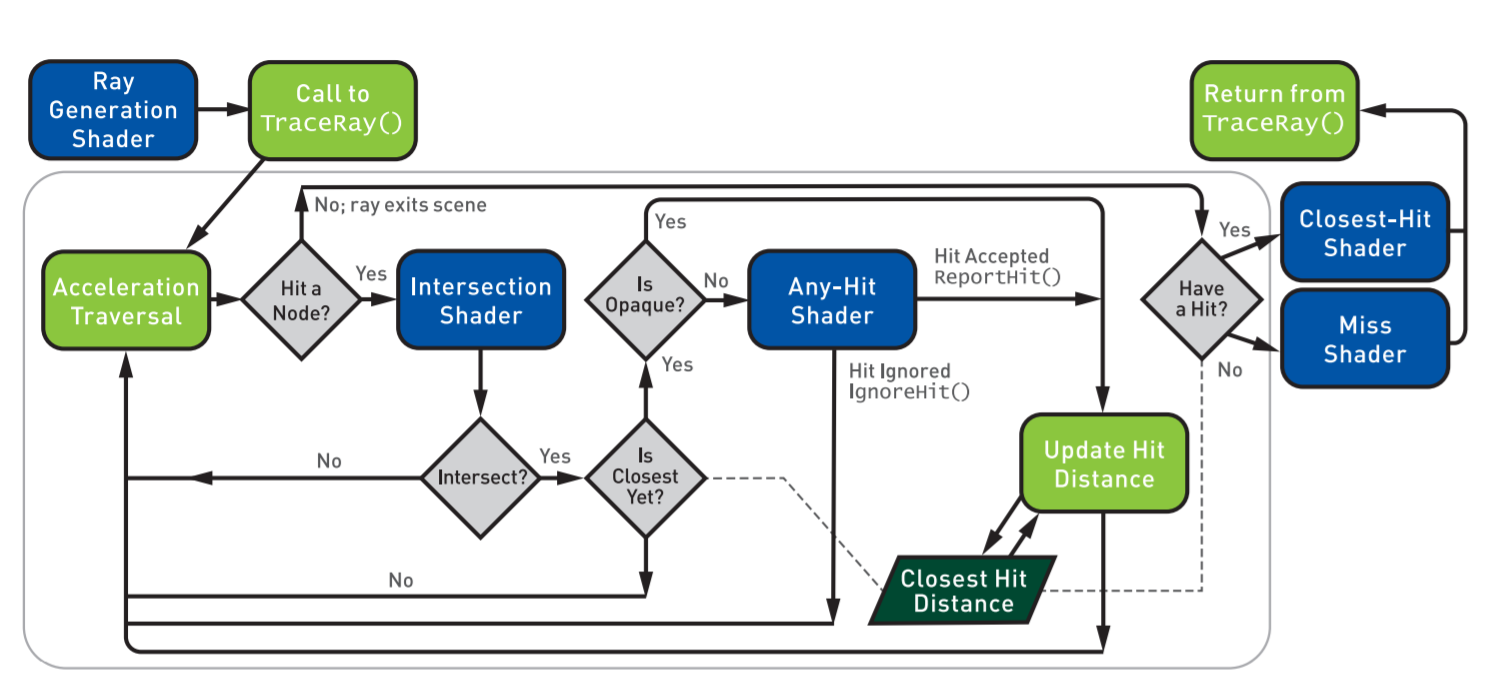
\includegraphics[width=\linewidth]{content/PathTracer/Bilder/DirectXRaytracingPipeline.png}
    \caption{DirectX Raytracing Pipeline aus \cite{Haines2019}}
    \label{pic:DirectXRaytracingPipeline}
\end{figure}

In \ref{pic:DirectXRaytracingPipeline} lässt sich der Beginn (Generierung eines Strahles) der neuen Pipeline
durch den programmierbaren \textbf{Ray Generation shader} erkennen.

\begin{algorithm}[H]
    \caption{Beispielhafter minimalistischer Ray Generation Shader}
    \begin{algorithmic}[1]
        \State [shader(\dq raygeneration \dq)]
        \State launchIndex = DispatchRaysIndex().xy;
        \For{(int i = 0; i < numberOfRays;i++)}
            \State float shadowRayMult = TraceRay(gRtScene,
            RAY\_FLAG\_ACCEPT\_FIRST\_HIT \_AND\_END\_SEARCH |
            RAY\_FLAG\_SKIP\_CLOSEST\_HIT\_SHADER,
            0xFF, 0, hitProgramCount, 0, ray, payload);
            \State float indirectRayColor = TraceRay(gRtScene, 0, 0xFF, 1, hitProgramCount, 1, rayColor, payload);
            \State color = shadowRayMult * shadingColor + computeindirectLighting(indirectRayColor);
        \EndFor
        \State output[id] = color;
    \end{algorithmic}
    \label{alg:Ray Gen}
\end{algorithm}

Mit Hilfe der Methode \textbf{TraceRay()} werden dann zur Beleuchtungsberechnung 
die Strahlen verschossen. Damit diese Methode richtig arbeiten kann übergeben wir neben unseren Strahl 
unter Anderem  unsere Szene inklusive Beschleunigungsstruktur, rayflags 
(beeinflussen Transparaenz, Culling, Abbruch)\cite{RayFlags} und einen payload.
Mit dem \textit{$payload_t$} Typ können wir einen struct mit Informationen jedem einzelnen Strahl mitgeben.

\begin{algorithm}[H]
    \caption{beispielhafter payload}
    \begin{algorithmic}[1]
        \State struct RayPayload = {
            \State        float4 color, uint32 seed, uint32 depth
            \State };
        \end{algorithmic}
        \label{alg:payload}
    \end{algorithm}
    
Diese Methode \textbf{TraceRay()} kann auch innerhalb der anderen Shader zum weiteren verschießen
von Strahlen verwendet werden. Beispiel beim Verschiessen vom Schattenstrahl: Flags 
RAY\_FLAG\_ACCEPT\_FIRST\_HIT\_AND\_END\_SEARCH, \newline
RAY\_FLAG\_SKIP\_CLOSEST\_HIT\_SHADER setzen, um unnötige 
Shadingberechnungen und weitere Schnittpunktberechnungen zu umgehen und mit einem Bit als payload 
die Sichtbarkeit zur Lichtquelle mitgeben.


Mit diesem beispielhaften payload können wir die Farbe akkumulieren, unseren verwendeten 
seed verwenden um z.B eine weiteren Strahlenschuss in einem Any-Hit Shader zu verwirklichen,  
solange die mit übergebene Rekursionstiefe in unserem payload eingehalten wird.  

\textbf{Intersection shader} führt die Schnittberechnungen durch.
Haben wir eine Szene, welche aus ausschließlich Dreiecken besteht, können wir
die auf Hardware standardmäßig gelieferte Implementierung übernehmen. 
Optionale Berechnungen für andere Geometrie können hier implementiert werden.
Bei einem gefundenen nähsten Schnittpunkt einer durchsichtigen Oberfläche wird der 
\textit{Any-hit shader} aufgerufen.
\textbf{Any-hit shaders} erlauben klassische \textit{Discards} oder informieren
über einen korrekten Schnitt. So können wir z.B. einen Alpha Test durchführen.

\begin{algorithm}[H]
    \caption{Any-Hit shader}
    \begin{algorithmic}[1]
        \State [shader(\dq anyhit \dq)]
        \If{(!alphaTest)} 
        \State IgnoreHit();
        \EndIf
    \end{algorithmic}
    \label{alg:any hit}
\end{algorithm}

Der \textbf{Closest-hit shader} berechnet den Schnittpunkt des Strahls mit der Geometrie
der Szene, die dem Strahlursprung am nähesten ist.
Mit der Kennzeichnung [shader(\dq closesthit \dq)] wird die Hauptmethode zur 
dessen Ausführung markiert. An dieser Stelle bietet es sich an die Shading Farbe 
mit der Schnittpunktinformation zu aktualisieren und/oder um eine Rekursionstiefe weiter 
zu gehen einen weiteren Strahl zu verschießen. 
Der \textbf{miss shader} wird immer dann ausgeführt, wenn ein Strahl die
Szenengeometrie nicht schneidet. Kann also für das Nachschauen in einer 
Environment Map verwendet werden. Im Folgenden \nameref{alg:Path Tracer Konzept}
nochmal vereinfacht in Pseudocode dargestellt, wobei die entsprechenden shader
im jeweiligen Codeabschnitt markiert sind.

\begin{algorithm}[H]
    \caption{Path Tracing Algorithmus}
    \begin{algorithmic}[1]
        \Procedure{Trace Path}{$BVH$}\Comment{verfolge Pfad durch Szene}
        \For{(x,y) $\in$ frame}
        \State strahl = verschiesseStrahlInPixel(x,y); // \textbf{ray generation shader}
        \For{blatt = bekommeBVHBlatt()}
        \State schnittpunkt = schneideGeometrie(strahl, blatt); //\textbf{Intersection shader}
        \If{schnittpunkt $\leq$ nähesterSchnittpunkt}
        \State aktualisiereNähestenSchnittpunkt();
        \EndIf
        \EndFor
        \If{Schnittpunkt gefunden}
        \State frame(x,y) = gebeFarbe(strahl,nähesterSchnittpunkt); //\textbf{closest-hit shader}
        \Else
        \State frame(x,y) = Umgebungskarte(x,y);//\textbf{miss shader}
        \EndIf
        \EndFor
        \EndProcedure
    \end{algorithmic}
    \label{alg:Path Tracer Konzept}
\end{algorithm}

\subsection{RenderGraph}

\begin{figure}[H]
    \centering
    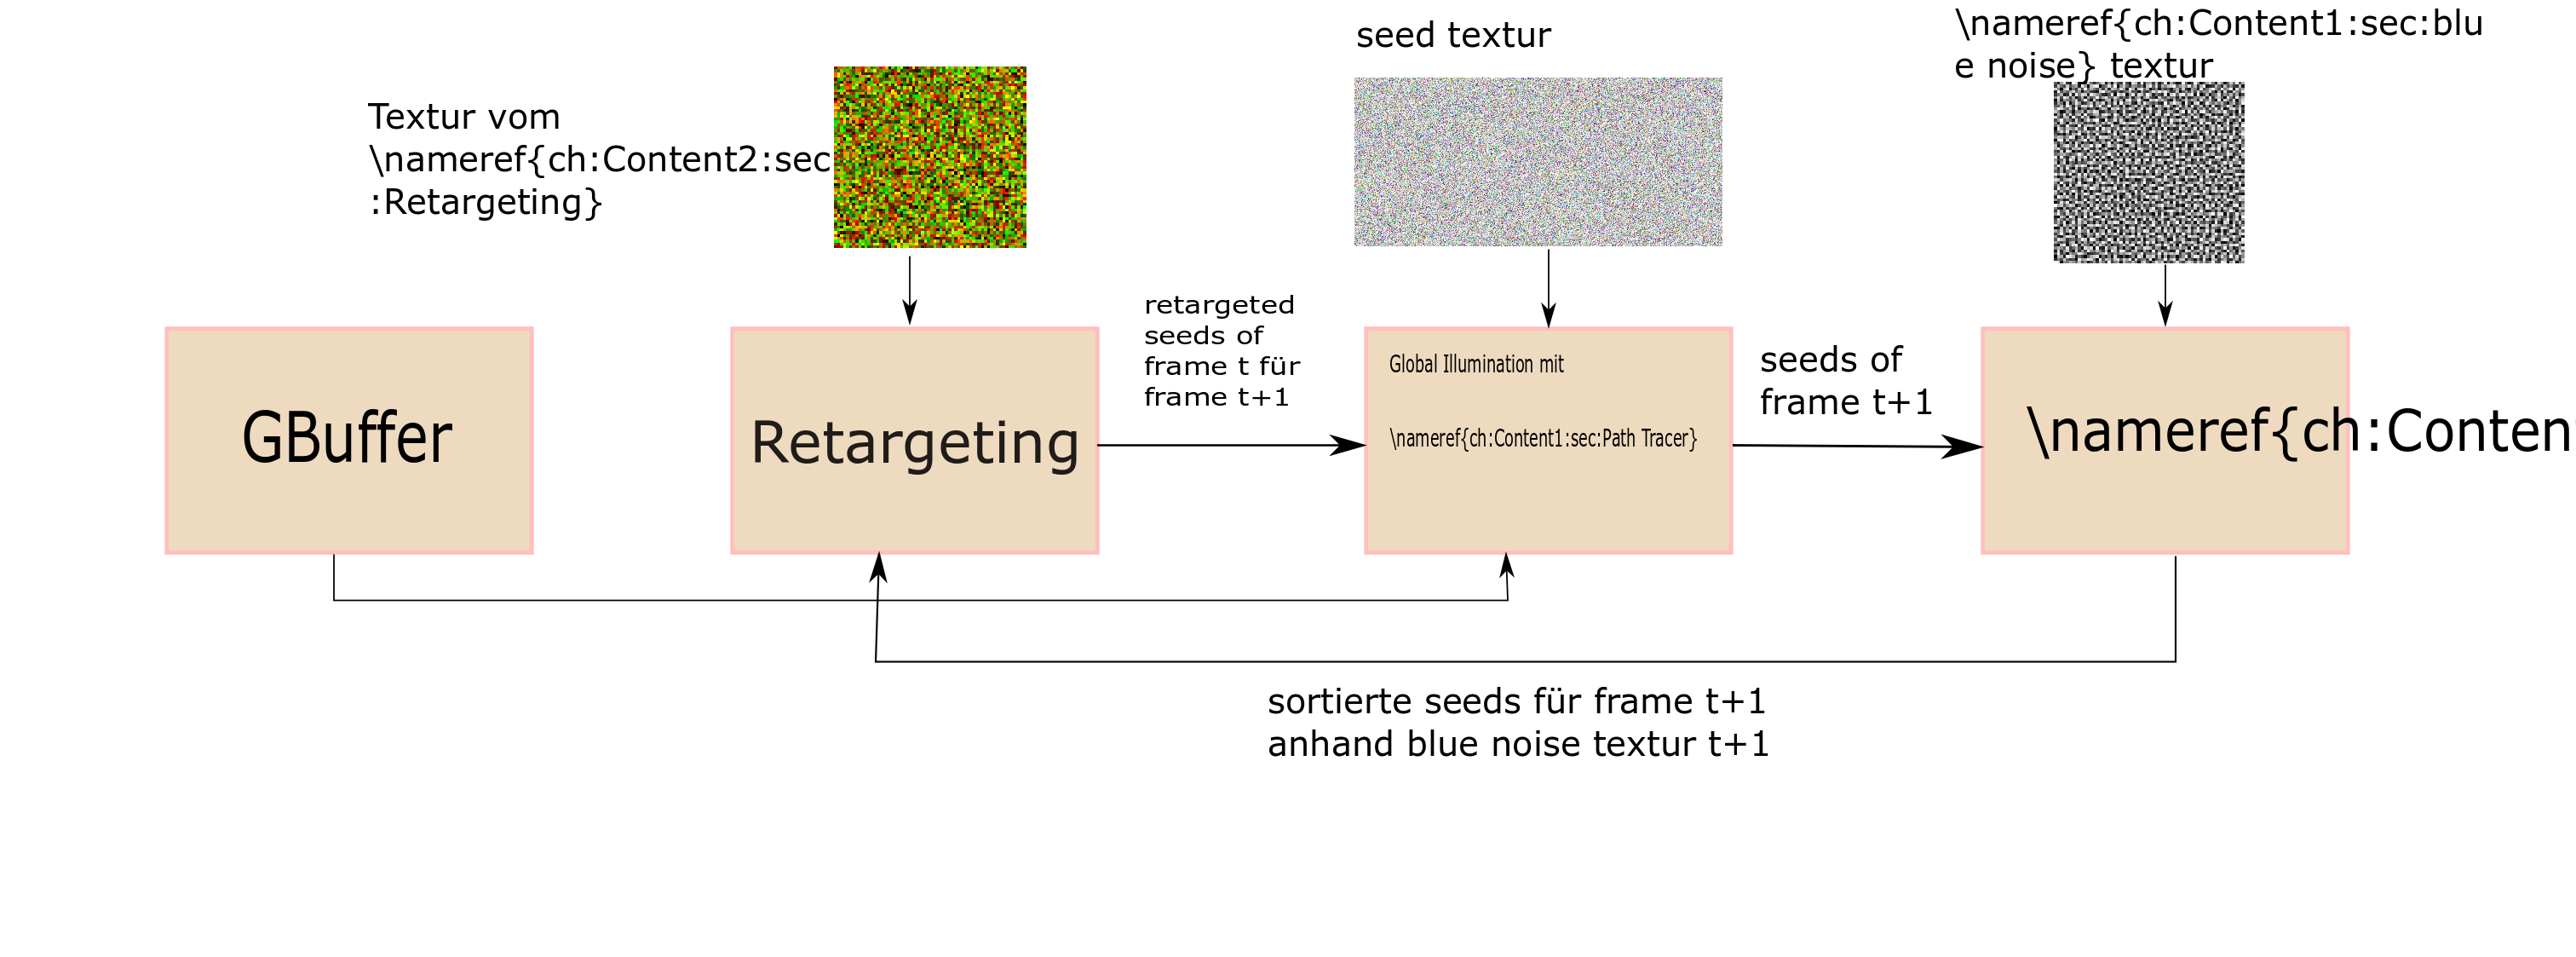
\includegraphics[width=\linewidth]{content/PathTracer/Bilder/render_graph.png}
    \caption{Unser Render Graph}
    \label{pic::RenderGraph}
\end{figure}





%% ===========================


%% ===========================
\newpage
\section{Blue Noise}
\label{ch:Content1:sec:BlueNoise}
\subsection{Eigenschaften}

Wie in \cite{Pet17} vorgestellt, macht man sich die Eigenschaften einer
blue noise Textur zu Nutze. Dabei werden im Folgenden, die dort bereit 
gestellten blue noise verteilten Texturen verwendet, welche anhand des in
\cite{ulichney1993void} vorgestellten Algorithmus erstellt wurden.
Die korrespondierenden Spektren werden mit Hilfe von \cite{FFTProgWeb} erstellt.

\subsubsection{Uniformität}
Die Uniformität(lat. \textit{uniformitas}-Einförmigkeit) garantiert uns 
wie in \cite{3288} eine gleichverteilte Wahrscheinlichkeitsdichtefunktion
mit zugehöriger gleichverteilter Wahrscheinlichkeitsfunktion. In \cite{Pet17}
sieht sie wie folgt aus: 

\begin{equation}\label{eq:uniformität}
    P(n \leq p) = p
\end{equation}

\cite{kiencke2009signale}

\subsubsection{Niedrige Frequenzen}
Niedrige Frequenzen sind in einer blue noise sehr wenig bis gar nicht 
vertreten. Dies ist an dem schwarzen Ring innerhalb der Fouriertransformierten
zu erkennen\ref{pic:blueNoiseFFT}.

\begin{figure}[H]\label{pic:blueNoiseFFT}
    \centering
    \begin{minipage}[t]{0.45\linewidth}
        \centering
        
\includegraphics[width=\linewidth]{content/BlueNoise/Bilder/LDR_LLL1_0.png}
        \caption{$512^{2}$ blue noise Textur}
    \end{minipage}
    \hfill
    \begin{minipage}[t]{0.45\linewidth}
        \centering
        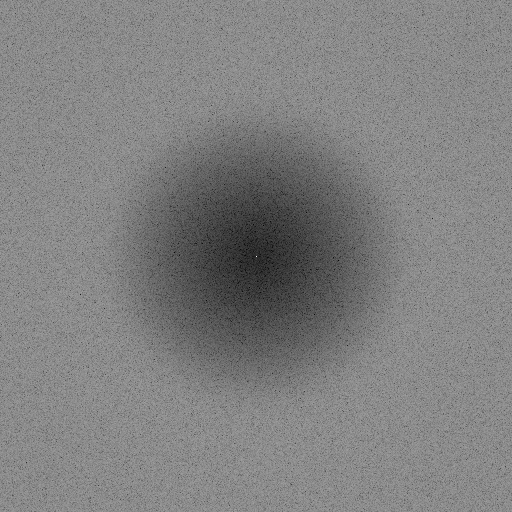
\includegraphics[width=\linewidth]{content/BlueNoise/Bilder/FFT_LDR_LLL1_0.png}
        \caption{Fourier Spektrum $512^{2}$ blue noise Textur}
    \end{minipage}
\end{figure}

\begin{figure}[H]\label{pic:bayerPatternFFT}
    \centering
    \begin{minipage}[t]{0.45\linewidth}
        \centering
        
\includegraphics[width=\linewidth]{content/BlueNoise/Bilder/BayerMatrix.png}
        \caption{$512^{2}$ bayer pattern Textur}
    \end{minipage}
    \hfill
    \begin{minipage}[t]{0.45\linewidth}
        \centering
        
\includegraphics[width=\linewidth]{content/BlueNoise/Bilder/FFT_BayerMatrix.png}
        \caption{Fourier Spektrum $512^{2}$ bayer pattern Textur}
    \end{minipage}
\end{figure}

\begin{figure}[H]\label{pic:tiledBlueNoiseFFT}
    \centering
    \begin{minipage}[t]{0.45\linewidth}
        \centering
        
\includegraphics[width=\linewidth]{content/BlueNoise/Bilder/BlueNoise64Tiled.png}
        \caption{$512^{2}$ bayer pattern Textur}
    \end{minipage}
    \hfill
    \begin{minipage}[t]{0.45\linewidth}
        \centering
        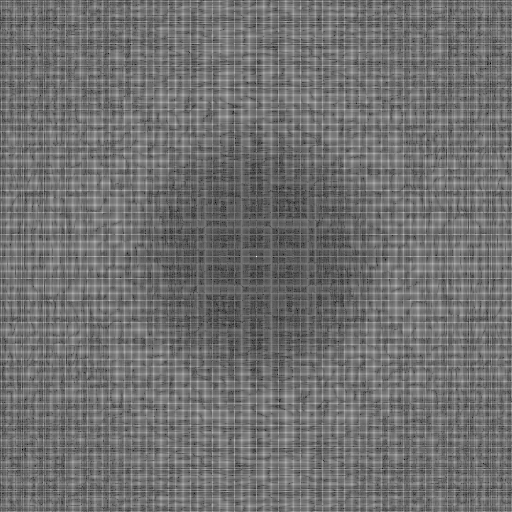
\includegraphics[width=\linewidth]{content/BlueNoise/Bilder/FFT_BlueNoise64Tiled.png}
        \caption{Fourier Spektrum $512^{2}$ bayer pattern Textur}
    \end{minipage}
\end{figure}

\subsubsection{Isotropie}
Die Isotropie(altgr. \textit{isos}-gleich und \textit{tropos}-Richtung)
einer blue noise Textur wird ausgenutzt. Dabei haben wir in allen
Dimensionen (in dieser Arbeit werden Texturen mit zwei benutzt) 
die Unabhängigkeit einer Eigenschaft. 


\subsubsection{Kachelung}
Eine weitere nützliche Eigenschaft der blue noise Verteilung ist die 
Möglichkeit der Kachelung. 
%% ===========================


%% ===========================
\newpage
\section{Quasi-Zufallsfolgen}
\label{ch:Content1:sec:QuasiRandomSequences}
\cite{owen1998scrambling} \cite{heitz:hal02150657}


\subsection{Einleitung}
Quasi-zufällige Sequenzen mit niedriger Abweichung sind deterministisch 
erzeugte Sequenzen, welche die Likelihood-Funktion der Clusterbildung

\begin{equation}\label{eq:Likeli-Hood-Gleichung}
    L_{x}(\delta) = f_{\delta}(x)
\end{equation}

minimieren. Dabei behalten wir die Eigenschaft einer zufälligen Folge, 
den gesamten Platz gleichmäßig auszufüllen. Diese Eigenschaften erinnern
uns an die besprochenen Eigenschaften bei \nameref{ch:Content1:sec:BlueNoise}.
Im Folgenden wird für uns der zweidimensionale Fall wichtig sein, weswegen
wir vom ein- über zum zweidimensionalen schauen werden.

\label{subsec:onedimensional}
\subsection{1-Dimension}
Diese Arbeit betrachtet Rekurrenz Sequenzen, basierend auf irrationalem 
Bruchrechnen der Form
\begin{equation}\label{eq:Rekurrenz Sequenz}
    R_{1}(\alpha) : t_n = s_0 + n\alpha(mod 1); n = 1,2,3,...
\end{equation}
wobei $\alpha \in \mathbb{I}$ und das (mod 1) einen \textit{"toroidally shift"}
bezeichnet. Will man mit dieser Formel eine Sequenz mit möglichst geringer
Abweichung schaffen, und genau das wollen wir, so wählen wir 
$\alpha = \Phi$ wobei $\Phi \approx 1.618033$ den goldenen Schnitt bezeichnet.
Wie \cite{quasirandomsequencesbyRoberts} gezeigt wird, ist diese Form von 
Sequenz die beste für das \nameref{eq:Rekurrenz Sequenz}.  

\subsection{2-Dimensionen}

Für mehrere Dimensionen, hier zwei, kombiniert man in gängigen Methoden 
einfach zwei \nameref{subsec:onedimensional} eindimensionale Sequenzen.
Für unsere Zwecke untersuchen wir hier die Generalisierung des bereits 
zuvor beschriebenen goldenen Schnitts \nameref{subsec:onedimensional}, wie
hier \cite{krcadinac2006new} beschrieben. 
Die sogenannte Plastische Zahl in ist die Lösung der
Gleichung \nameref{eq:plastische Nummer}
\begin{equation}\label{eq:kubisch}
   x^{3} - x - 1 = 0
\end{equation}
Die Lösung dieser Gleichung lässt sich über die Padovan und Perrin Sequenz
definieren. Damit erhalten wir Plastische Zahl $\Phi$:

\begin{equation} \label{eq:plastische Nummer}
   \Phi = \frac{(9 - \sqrt{69})^{1/3} + (9 + \sqrt{69})^{1/3}}
               {2^{1/3}3^{2/3}} \approx 1.32471795
\end{equation}

\cite{vanderlaanplasticnumber}
\cite{wolframalphaPlastic}
Folgende Gleichung ist auch einfach erweiterbar für höhere Dimensionen.
\begin{equation}\label{eq:1 zu N - Dimensional}
    t_{n} = n\alpha(mod 1), n = 1,2,3,..
    \alpha = (\frac{1}{\Phi_{d}}, \frac{1}{\Phi_{d}^{2}}),
\end{equation}
Dabei ist $\Phi_{d}$ der goldene Schnitt. $\Phi_{d}^{2}$ ist Lösung der
\nameref{eq:kubisch} obigen Gleichung.


\cite{quasirandomsequencesbyRoberts}
\begin{lstlisting}[style=CStyle]
   float g = 1.32471795724474602596; //Plastische Zahl
   float a1 = 1.0/g;
   float a2 = 1.0/(g*g);
   x[n] = (0.5+a1*n) %1; //toroidally shifted
   y[n] = (0.5+a2*n) %1; //toroidally shifted
\end{lstlisting}


\subsection{Dither Texturen und quasi-zufällige Folgen}

%% ===========================



%% content.tex
%%

%% ==============
\newpage
\chapter{Temporaler Algorithmus}
\label{ch:TemporalerAlgorithmus}
In diesem Abschnitt wird auf den in \cite{hal02158423} vorgestellten, temporalen Algorithmus eingegangen.
Dieser besteht grundsätzlich aus den beiden Schritten: \nameref{ch:Content2:sec:Sorting} und  
\nameref{ch:Content2:sec:Retargeting}. Wir werden die gewonnenen Erkenntnisse (siehe Kapitel \ref{ch:Grundlagen})
nutzen um eine zeitlich stabile \nameref{ch:Content1:sec:blue noise} Fehlerverteilung im Bildraum zu erreichen.
Der benutzte \nameref{ch:Content1:sec:Path Tracer} benutzt zufällig generierte Anfangswerte 
(siehe \cite{matsumoto1998mersenne}). Der darauffolgende Schritt sortiert diese Anfangswerte anhand 
einer \nameref{ch:Content1:sec:blue noise} Textur, auf die mit Hilfe einer quasi-zufälligen Sequenz 
\ref{ch:Content1:sec:Quasi-Zufallsfolgen} zugegriffen wird. Bevor diese sortierten Anfangswerte 
zum Rendern des nächsten Bildes benutzt werden durchlaufen Sie noch eine Permutation 
(siehe Abschnitt \ref{ch:Content2:sec:Retargeting}).
Desweiteren sollte man beachten, dass für diesen Algorithmus Annahmen getroffen wurden, auf deren Ursache im darauffolgenden 
Abschnitt \ref{ch:Content2:sec:a Posteriori} eingegangen wird:
Der Algorithmus arbeitet Blockweise auf den Pixeln und erwartet, dass benachbarte
Pixel innerhalb dieses Blockes den selben Wert haben. Da wir einen temporalen Algorithmus haben, soll diese Annahme 
auch über mehrere gerenderte Bilder hinweg gelten. Es sollte also beachtet werden, dass der Algorithmus z.B. nicht 
für Objektkanten oder ruckartige Bewegungen (der Kamera oder Objekte) ausgelegt ist.

\begin{figure}[H]
    \begin{subfigure}{\textwidth}
        \centering 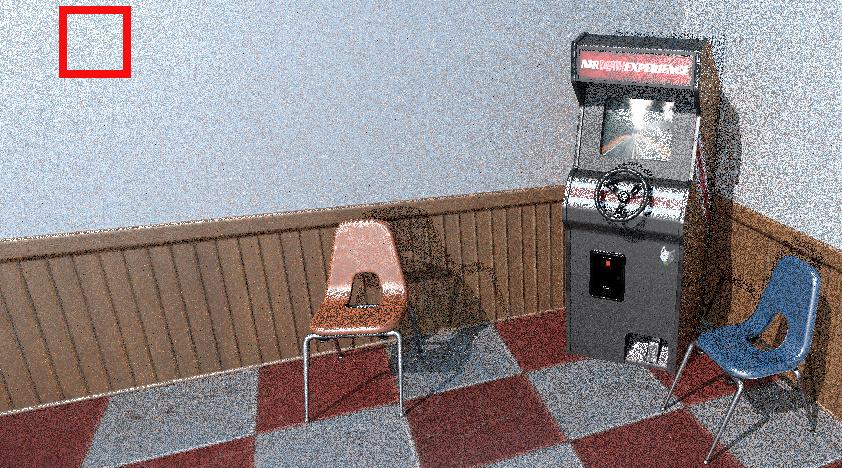
\includegraphics[width=0.7\linewidth]{content/TemporalerAlg/Bilder/WhiteNoise/white_noise_ausschnitt.png}
        \caption{Szene}
        \label{fig:Szene_Weißes Rauschen}
    \end{subfigure}
    \begin{subfigure}{0.5\textwidth}
        \centering 
\includegraphics[width=0.5\linewidth]{content/TemporalerAlg/Bilder/WhiteNoise/white_noise_64x64.jpg} 
        \caption{Szenenausschnitt}
        \label{fig:ausschnitt_Weißes_Rauschen}
    \end{subfigure}
    \begin{subfigure}{0.5\textwidth}
        \centering 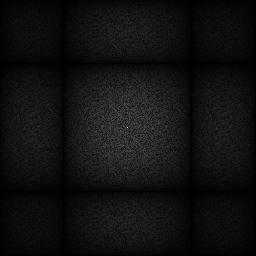
\includegraphics[width=0.5\linewidth]{content/TemporalerAlg/Bilder/WhiteNoise/white_noise_64x64_fourier.png}
        \caption{Fouriertransformierte des Ausschnitts}
        \label{fig:Fouriertransformierte_Weißes_Rauschen}
    \end{subfigure}
        \caption{Ausgangssituation; Erzeugtes Bild mit zufälligen Seeds ohne temp. Alg.}
        \label{fig:Path Tracer mit zufälligen Seeds}
\end{figure}

In Abbildung \ref{fig:Path Tracer mit zufälligen Seeds} sehen wir die Ausgabe des \nameref{ch:Content1:sec:Path Tracer}
mit zufälligen Anfangswerten(Mersenne-Twister) weder mit dem Sortier \ref{ch:Content2:sec:Sorting} noch dem 
\nameref{ch:Content2:sec:Retargeting} Schritt. Der Szenenausschnitt lässt deutliche Clusterbildungen erkennen und auch
die Betrachtung des Spektrums lässt auf eine white noise \ref{pic:white noise} Verteilung schließen.

%% ==============



%% ===========================
\section{Sorting}
\label{ch:Content2:sec:Sorting}
\todo{replace dummy code with correct code}
\cite{hal-02158423}
\begin{algorithm}
    \caption{\textbf{Sortier Schritt t} nach dem Rendern von Frame t
    und vor dem Rendern von Frame t+1}
    \begin{algorithmic}[1]
        \STATE pixel \textbf{consists of} value,index;
        \STATE List framePixelsIntensities, noiseIntensities;
        \STATE List L $\leftarrow$ pixels in block
        \STATE //init lists
        \FORALL{(i,j) $\leftarrow$ L} 
        \STATE framePixelsIntensities(i,j) = pixelIntensity(frame(i,j));
        \STATE noiseIntensities(i,j) = pixelIntensity(blueNoise(i,j));
        \ENDFOR \newline
        
        \STATE //sort the two lists by means of intensities
        \STATE sort(framePixelsIntensities);
        \STATE Sort(noiseIntensities); \newline

        \STATE //now we reorder our seeds hence the sorted lists
        \FORALL{$i = 1 .. numberOfPixelsPerBlock$}
        \STATE $sortedSeeds(noiseIntensities.getIndex(i)) = incomingSeeds(framePixelIntensities.getIndex(i))$;
        \ENDFOR
    \end{algorithmic}
    \label{alg:Sortier}
\end{algorithm}
%% ===========================



%% ===========================
\section{Retargeting}
\label{ch:Content2:sec:Retargeting}
Zu Grunde liegender Sinn dieses Schrittes: Vertauschen der Seeds, die 
verteilt sind wie $BlueNoise_{t}$ , aufgrund des zuvor ausgeführten Sortierschrittes \ref{ch:Content2:sec:Sorting}
, sodass Sie verteilt sind wie die Textur
$BlueNoise_{t+1}$. Aufgrund dessen haben wir eine Aufsummierung der
blue noise Fehlerverteilungen über die ersten paar Frames(siehe \nameref{fig:Retargeting_And_Sorting_Szene_t1}).

\begin{algorithm}[H]
    \caption{\textbf{Retargeting Schritt}}
    \begin{algorithmic}[1]
        \State //permutation indices from precomputed texture
        \State $retaget_{t}$ = retarget\_texure[calc\_correct\_offset()];
        
        \State $retargetedSeeds(old\_id + retaget_{t}) = incomingSeeds(old\_id);$
        
    \end{algorithmic}
    \label{alg:retargetingAlg}
\end{algorithm}

\begin{figure}[H]\label{pic:Permutation}
    \centering
    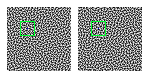
\includegraphics[width=0.5\linewidth]{content/simulatedAnnealing/Bilder/Permutation.png}
    \caption{Permutation}
\end{figure}

\newpage
%%%%%%%%%%%%%%%%%%%%%%%%%%%%%%%%%%%%%%%%%%%%%%%%%%%%%%%%%%%%
%%%%%%%%%% Beginning the Sequence of getting to blue noise from white noise
%%%%%%%%%%%%%%%%%%%%%%%%%%%%%%%%%%%%%%%%%%%%%%%%%%%%%%%%%%%%
\label{fig:Retargetbilderstrecke}
\begin{figure}[H]

    \begin{subfigure}{\textwidth}
        \centering 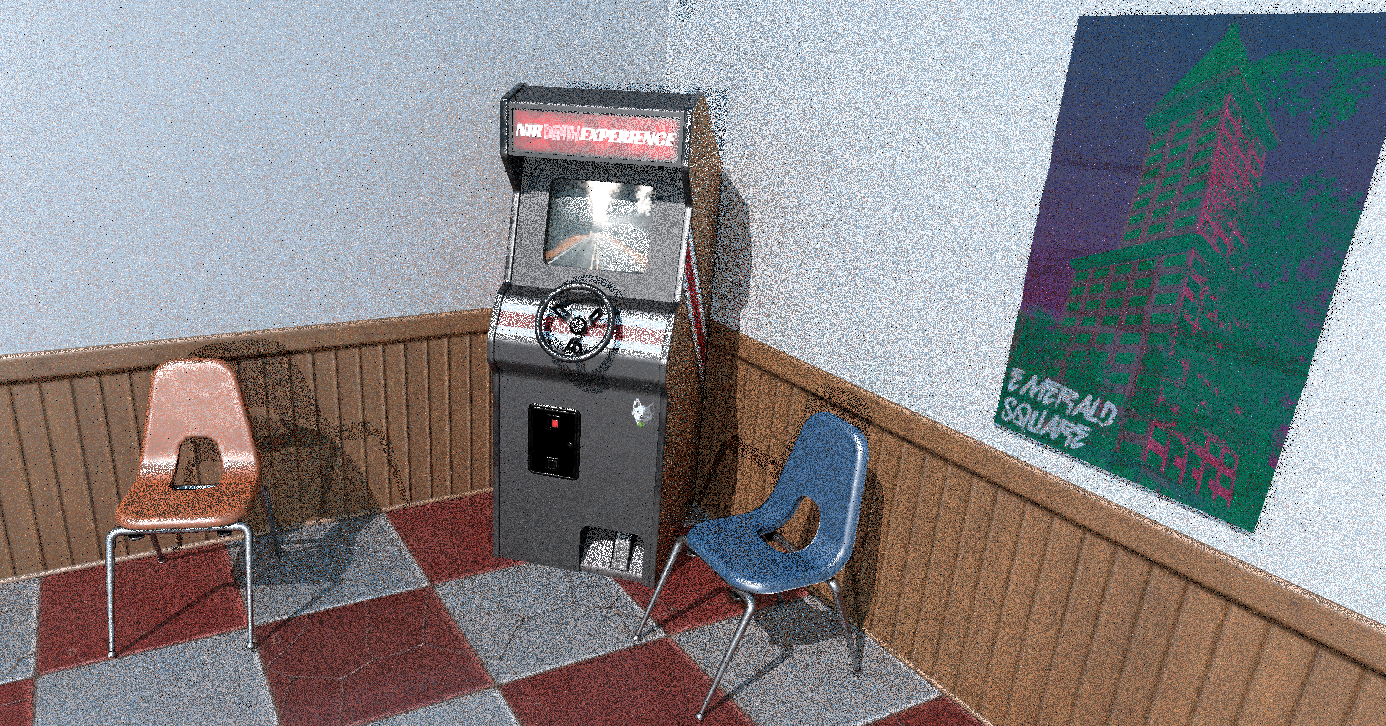
\includegraphics[scale=.25]{content/TemporalerAlg/Bilder/Retargeting/Screenshots/seed_debug_3.0_selection.png}
        \caption{Szene}
        \label{fig:Retargeting_And_Sorting_Szene_t1}
    \end{subfigure}
    \begin{subfigure}{0.5\textwidth}
        \centering 
\includegraphics[width=0.4\linewidth]{content/TemporalerAlg/Bilder/Retargeting/Screenshots/seed_debug_3.0_ausschnitt.png} 
        \caption{Szenenausschnitt}
        \label{fig:Retargeting_And_Sorting_ausschnitt_t1}
    \end{subfigure}
    \begin{subfigure}{0.5\textwidth}
        \centering 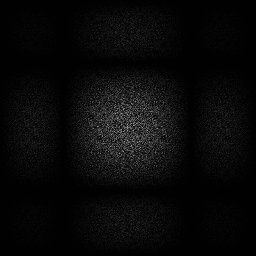
\includegraphics[width=0.4\linewidth]{content/TemporalerAlg/Bilder/Retargeting/Screenshots/Spektren/seed_debug_3.0_ausschnitt.png}
        \caption{Fouriertransformierte des Ausschnitts}
        \label{fig:Retargeting_And_Sorting_Fouriertransformierte_t1}
    \end{subfigure}
        \caption{Zeitpunkt t=1}
        \label{fig:Retargeting_And_Sorting_Verlauf_t1}
\end{figure}

\begin{figure}[H]
    \begin{subfigure}{\textwidth}
        \centering 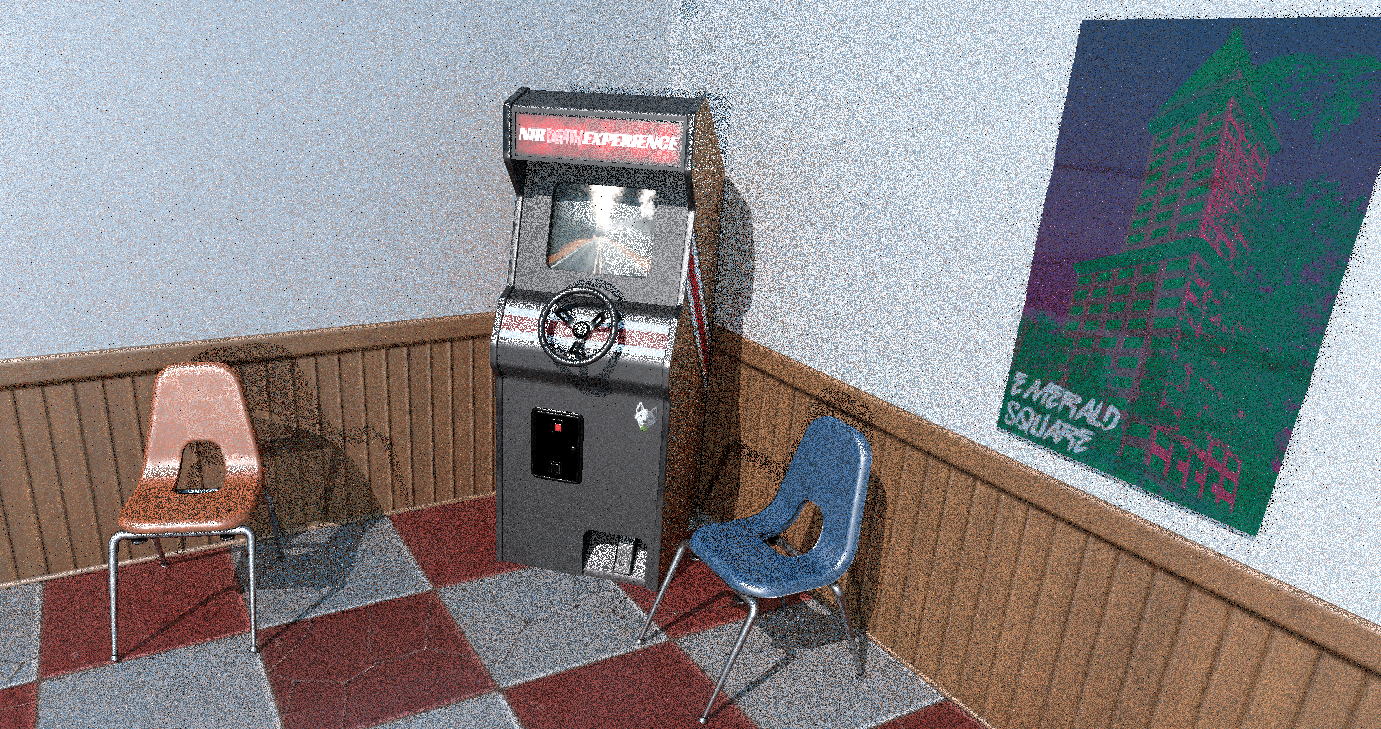
\includegraphics[scale=.25]{content/TemporalerAlg/Bilder/Retargeting/Screenshots/seed_debug_4.0_selection.png}
        \caption{Szene}
        \label{fig:Retargeting_And_Sorting_Szene_t2}
    \end{subfigure}
    \begin{subfigure}{0.5\textwidth}
        \centering
\includegraphics[width=0.4\linewidth]{content/TemporalerAlg/Bilder/Retargeting/Screenshots/seed_debug_4.0_ausschnitt.png} 
        \caption{Szenenausschnitt}
        \label{fig:Retargeting_And_Sorting_ausschnitt_t2}
    \end{subfigure}
    \begin{subfigure}{0.5\textwidth}
        \centering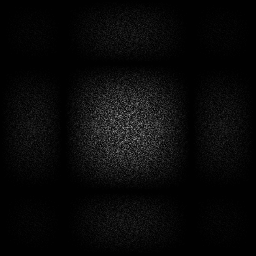
\includegraphics[width=0.4\linewidth]{content/TemporalerAlg/Bilder/Retargeting/Screenshots/Spektren/seed_debug_4.0_ausschnitt.png}
        \caption{Fouriertransformierte des Ausschnitts}
        \label{fig:Retargeting_And_Sorting_Fouriertransformierte_t2}
    \end{subfigure}
        \caption{Zeitpunkt t=2}
        \label{fig:Retargeting_And_Sorting_Verlauf_t2}
\end{figure}

\begin{figure}[H]
    \begin{subfigure}{\textwidth}
        \centering 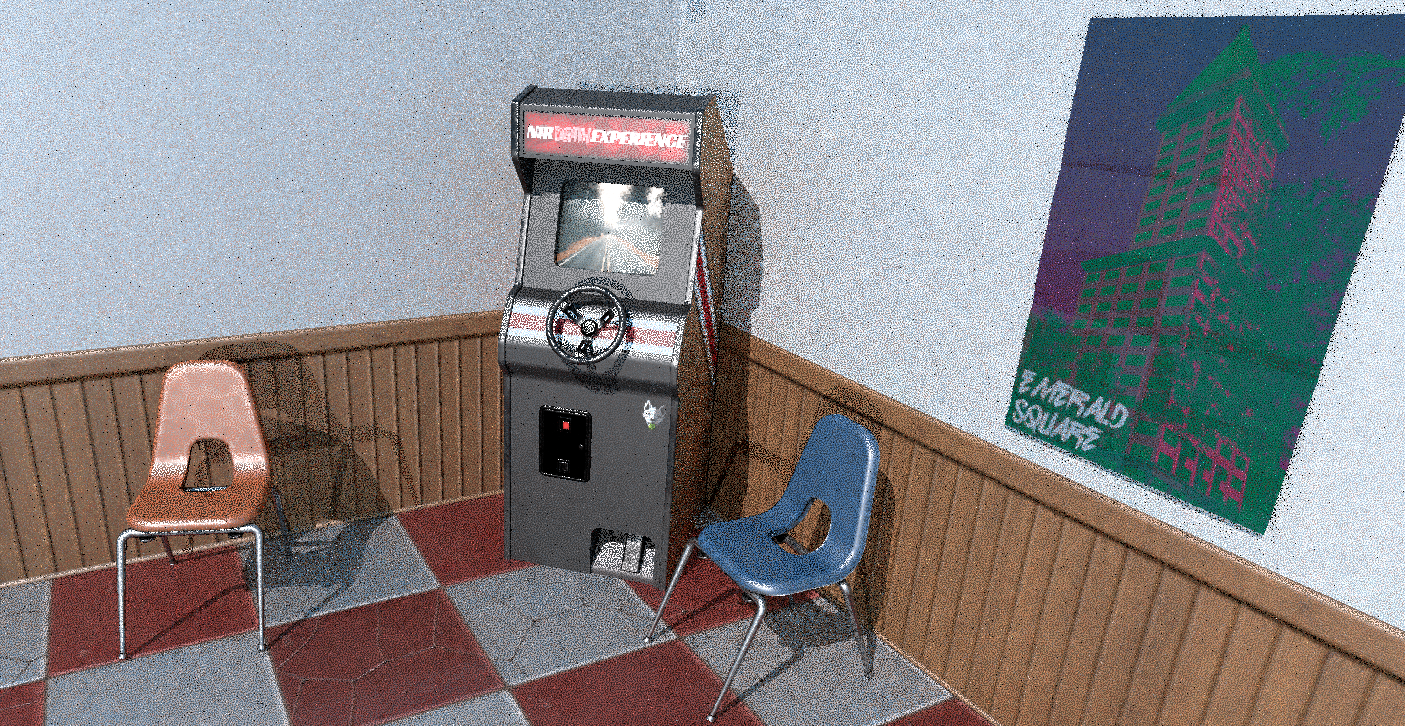
\includegraphics[scale=.25]{content/TemporalerAlg/Bilder/Retargeting/Screenshots/seed_debug_5.0_selection.png}
        \caption{Szene}
        \label{fig:Retargeting_And_Sorting_Szene_t3}
    \end{subfigure}
    \begin{subfigure}{0.5\textwidth}
        \centering
\includegraphics[width=0.4\linewidth]{content/TemporalerAlg/Bilder/Retargeting/Screenshots/seed_debug_5.0_ausschnitt.png} 
        \caption{Szenenausschnitt}
        \label{fig:Retargeting_And_Sorting_ausschnitt_t3}
    \end{subfigure}
    \begin{subfigure}{0.5\textwidth}
        \centering
\includegraphics[width=0.4\linewidth]{content/TemporalerAlg/Bilder/Retargeting/Screenshots/Spektren/seed_debug_5.0_ausschnitt.png}
        \caption{Fouriertransformierte des Ausschnitts}
        \label{fig:Retargeting_And_Sorting_Fouriertransformierte_t3}
    \end{subfigure}
        \caption{Zeitpunkt t=3}
        \label{fig:Retargeting_And_Sorting_Verlauf_t3}
\end{figure}

\begin{figure}[H]
    \begin{subfigure}{\textwidth}  
        \centering 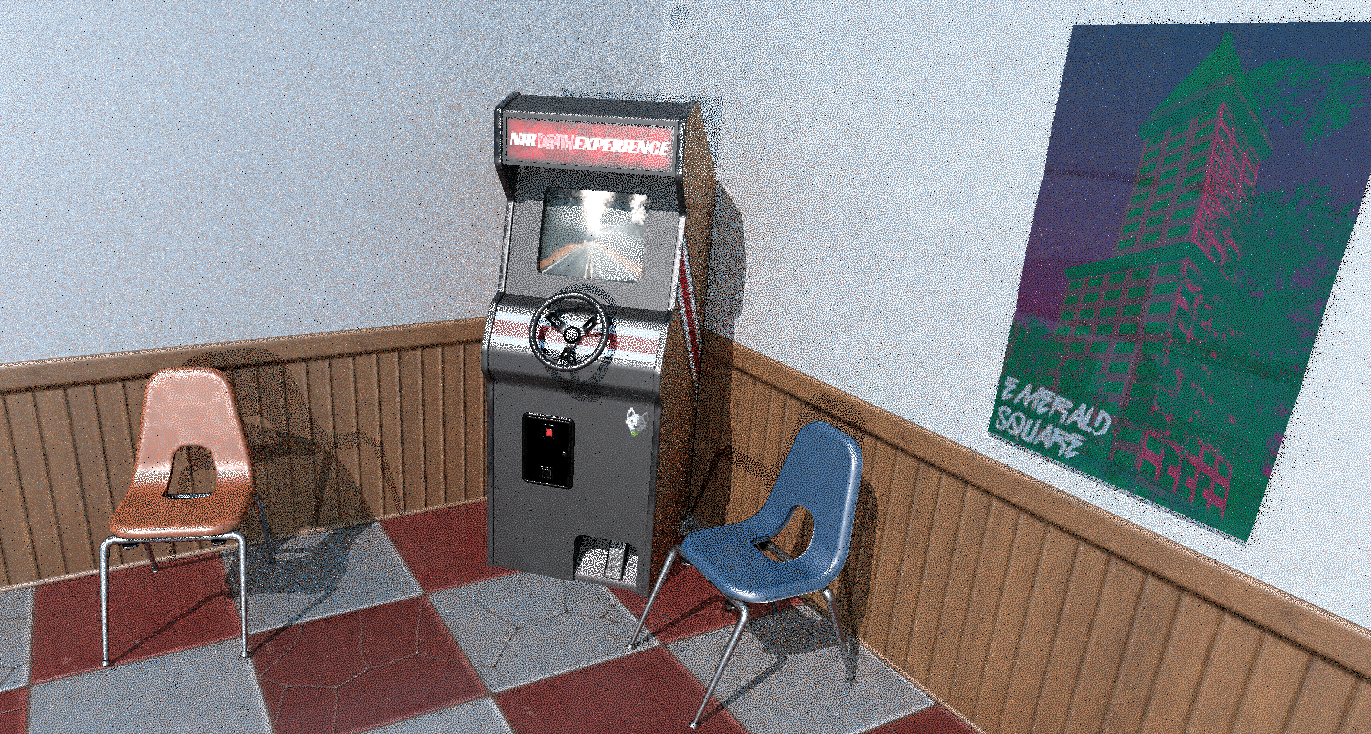
\includegraphics[scale=.25]{content/TemporalerAlg/Bilder/Retargeting/Screenshots/seed_debug_6.0_selection.png}
        \caption{Szene}
        \label{fig:Retargeting_And_Sorting_Szene_t4}
    \end{subfigure}
    \begin{subfigure}{0.5\textwidth}
        \centering
\includegraphics[width=0.4\linewidth]{content/TemporalerAlg/Bilder/Retargeting/Screenshots/seed_debug_6.0_ausschnitt.png} 
        \caption{Szenenausschnitt}
        \label{fig:Retargeting_And_Sorting_ausschnitt_t4}
    \end{subfigure}
    \begin{subfigure}{0.5\textwidth}
        \centering
\includegraphics[width=0.4\linewidth]{content/TemporalerAlg/Bilder/Retargeting/Screenshots/Spektren/seed_debug_6.0_ausschnitt.png}
        \caption{Fouriertransformierte des Ausschnitts}
        \label{fig:Retargeting_And_Sorting_Fouriertransformierte_t4}
    \end{subfigure}
        \caption{Zeitpunkt t=4}
        \label{fig:Retargeting_And_Sorting_Verlauf_t4}
\end{figure}

\begin{figure}[H]
    \begin{subfigure}{\textwidth}   
        \centering 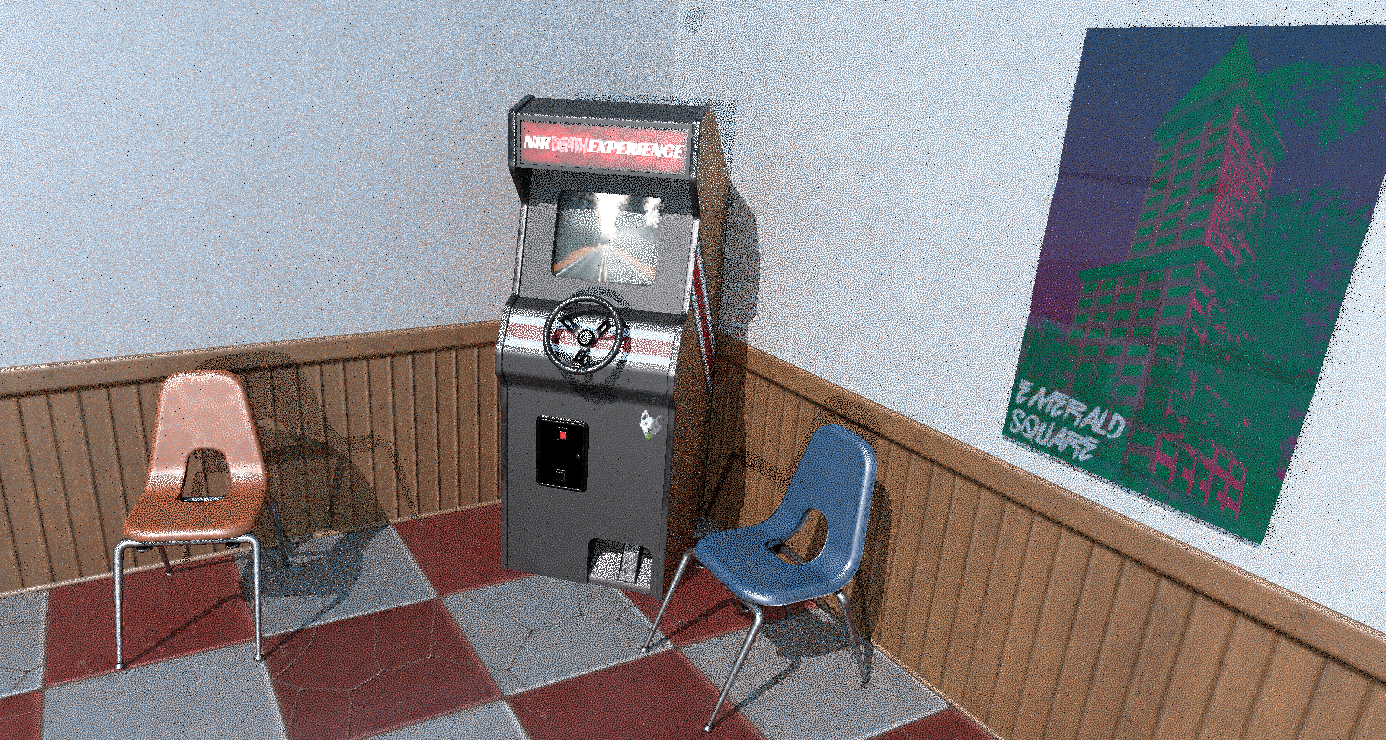
\includegraphics[scale=.25]{content/TemporalerAlg/Bilder/Retargeting/Screenshots/seed_debug_7.0_selection.png}
        \caption{Szene}
        \label{fig:Retargeting_And_Sorting_Szene_t5}
    \end{subfigure}
    \begin{subfigure}{0.5\textwidth}
        \centering
\includegraphics[width=0.4\linewidth]{content/TemporalerAlg/Bilder/Retargeting/Screenshots/seed_debug_7.0_ausschnitt.png} 
        \caption{Szenenausschnitt}
        \label{fig:Retargeting_And_Sorting_ausschnitt_t5}
    \end{subfigure}
    \begin{subfigure}{0.5\textwidth}
        \centering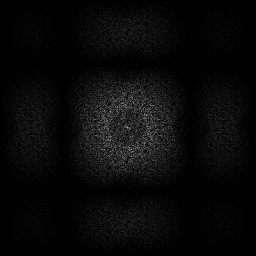
\includegraphics[width=0.4\linewidth]{content/TemporalerAlg/Bilder/Retargeting/Screenshots/Spektren/seed_debug_7.0_ausschnitt.png}
        \caption{Fouriertransformierte des Ausschnitts}
        \label{fig:Retargeting_And_Sorting_Fouriertransformierte_t5}
    \end{subfigure}
        \caption{Zeitpunkt t=5}
        \label{fig:Retargeting_And_Sorting_Verlauf_t5}
\end{figure}

\begin{figure}[H]
    \begin{subfigure}{\textwidth}   
        \centering 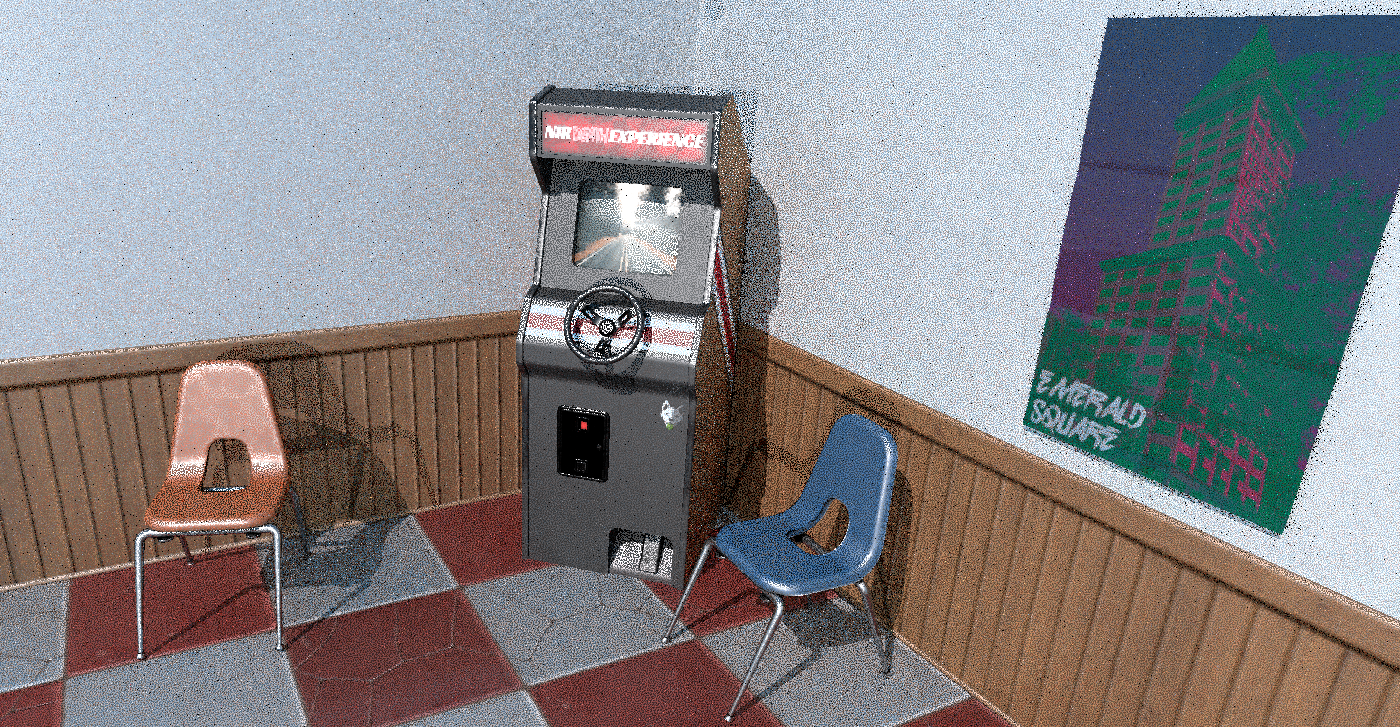
\includegraphics[scale=.25]{content/TemporalerAlg/Bilder/Retargeting/Screenshots/seed_debug_8.0_selection.png}
        \caption{Szene}
        \label{fig:Retargeting_And_Sorting_Szene_t6}
    \end{subfigure}
    \begin{subfigure}{0.5\textwidth}
        \centering
\includegraphics[width=0.4\linewidth]{content/TemporalerAlg/Bilder/Retargeting/Screenshots/seed_debug_8.0_ausschnitt.png} 
        \caption{Szenenausschnitt}
        \label{fig:Retargeting_And_Sorting_ausschnitt_t6}
    \end{subfigure}
    \begin{subfigure}{0.5\textwidth}
        \centering
\includegraphics[width=0.4\linewidth]{content/TemporalerAlg/Bilder/Retargeting/Screenshots/Spektren/seed_debug_8.0_ausschnitt.png}
        \caption{Fouriertransformierte des Ausschnitts}
        \label{fig:Retargeting_And_Sorting_Fouriertransformierte_t6}
    \end{subfigure}
        \caption{Zeitpunkt t=6}
        \label{fig:Retargeting_And_Sorting_Verlauf_t6}
\end{figure}

\begin{figure}[H]
    \begin{subfigure}{\textwidth}   
        \centering 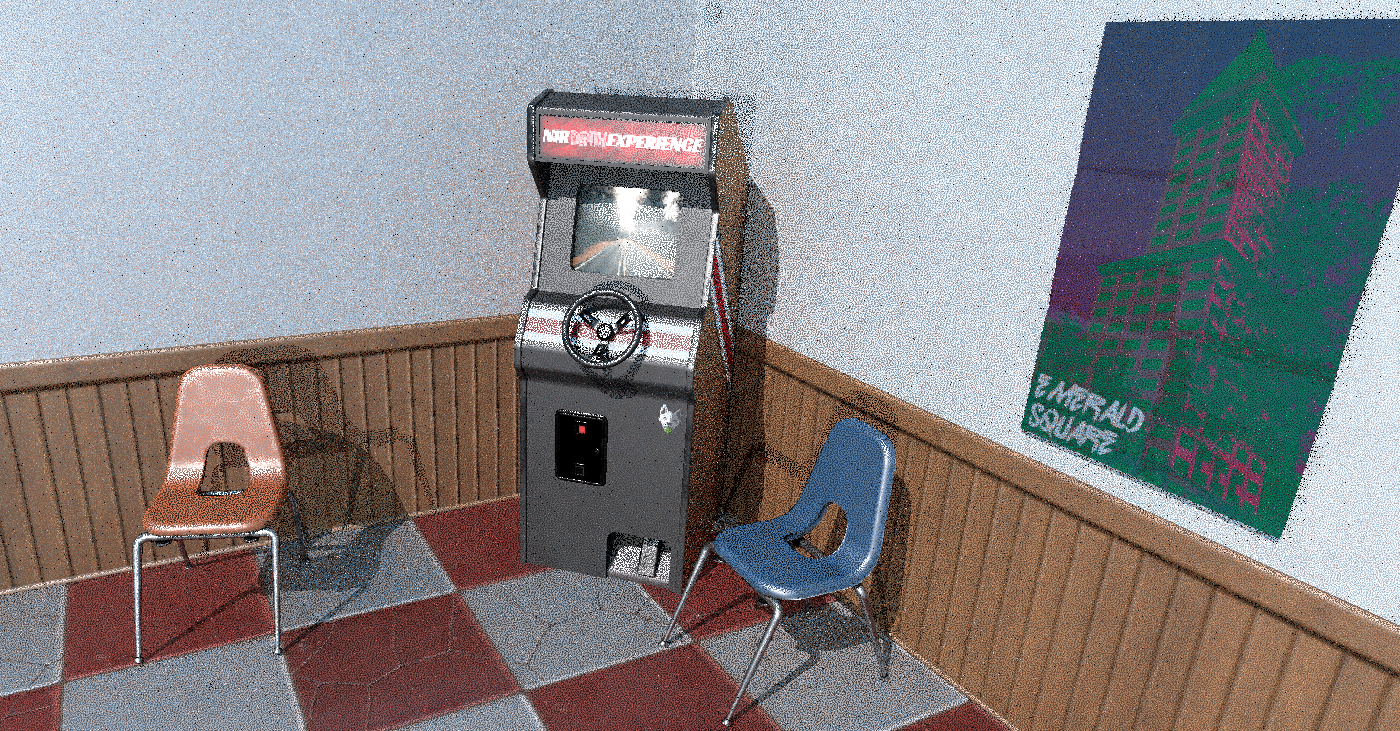
\includegraphics[scale=.25]{content/TemporalerAlg/Bilder/Retargeting/Screenshots/seed_debug_9.0_selection.png}
        \caption{Szene}
        \label{fig:Retargeting_And_Sorting_Szene_t7}
    \end{subfigure}
    \begin{subfigure}{0.5\textwidth}
        \centering
\includegraphics[width=0.4\linewidth]{content/TemporalerAlg/Bilder/Retargeting/Screenshots/seed_debug_9.0_ausschnitt.png} 
        \caption{Szenenausschnitt}
        \label{fig:Retargeting_And_Sorting_ausschnitt_t7}
    \end{subfigure}
    \begin{subfigure}{0.5\textwidth}
        \centering
\includegraphics[width=0.4\linewidth]{content/TemporalerAlg/Bilder/Retargeting/Screenshots/Spektren/seed_debug_9.0_ausschnitt.png}
        \caption{Fouriertransformierte des Ausschnitts}
        \label{fig:Retargeting_And_Sorting_Fouriertransformierte_t7}
    \end{subfigure}
        \caption{Zeitpunkt t=7}
        \label{fig:Retargeting_And_Sorting_Verlauf_t7}
\end{figure}


%% ===========================

